\newpage
\section{Ricostruzione dell'albero}
Se l'albero è binario, ogni nodo ha esattamente due figli, quindi la speciazione può essere vista come una divisione in due, e la matrice delle distanze prende il nome di \textit{distanza additiva}. 

Sia $T$ un albero binario senza radice, e $D$ la matrice ultrametrica delle distanze totali associata (si ricorda che $D$ è simmetrica). Si vuole calcolare l'albero $T$ che induce una matrice $D_T$ simile a $D$. 

\textit{Quando una matrice $M$ ha un albero $T$ che la induce?} Per capire se esiste l'albero, si controllano tutte le \textbf{quaterne} di punti.

$D$ è una distanza additiva se soddisfa la condizione dei 4 punti:
\begin{enumerate}
	\item $D[v, w] + D[x, y]$;
	\item $D[v, x] + D[w, y]$;
	\item $D[v, y] + D[w, x]$.
\end{enumerate}
Il massimo dei tre valori è ottenuto esattamente da due di questi tre casi. La condizione è anche inversa: se questa proprietà è soddisfatta, la distanza è additiva. 

Si ha la matrice $M$ associata a $T$, e si vuole ottenere una proprietà della matrice: l'idea di base è che le distanze non possano essere completamente slegate tra loro, ma rispettino la condizione dei quattro punti. 

\begin{figure}[H]
	\caption{Albero generico binario, distanza additiva}
	\centering
\begin{forest}
	for tree={circle, draw,minimum size=1.5em,s sep=1cm,
	every leaf node={
		draw,
		rectangle
	}},
	[
		[, edgelabel={left}{6}
			[, edgelabel={left}{6}, nodevalue={south}{A}],
			[, edgelabel={right}{5}, nodevalue={south}{F}]
		],
		[, edgelabel={right}{10}
			[, edgelabel={left}{2}, nodevalue={south}{D}],
			[, edgelabel={right}{9}
				[, edgelabel={left}{7}, nodevalue={south}{B}],
				[, edgelabel={right}{1}
					[, edgelabel={left}{2}, nodevalue={south}{C}],
					[, edgelabel={right}{3}, nodevalue={south}{E}]
				]
			]
		]
	]
\end{forest}
\end{figure}
In un albero, vengono estratte quattro specie (foglie), considerando soltanto la porzione di cammini che li collega. Essendo l'albero binario, la struttura sarà sempre la stessa. Sono poi considerate tutte le coppie di distanze: due di esse avranno un valore più elevato, e uno sarà minore. Questo accade perché per due coppie non sarà necessario attraversare il cammino intermedio. 

Per calcolare le distanze è sufficiente sfruttare la struttura dell'albero, non necessariamente i valori. Se un cammino ha etichetta 0, la disuguaglianza diventa uguaglianza, e per posizionarlo si contrae un arco.

\begin{figure}
	\caption{Condizione dei quattro punti}
	\centering
	

\tikzset{every picture/.style={line width=0.75pt}} %set default line width to 0.75pt        

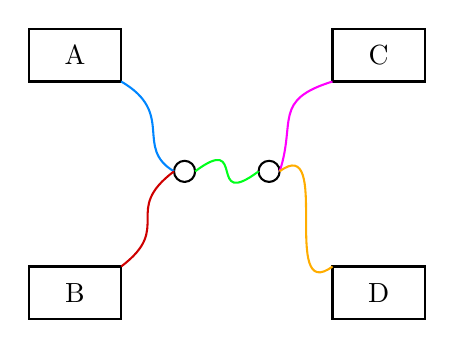
\begin{tikzpicture}[x=0.75pt,y=0.75pt,yscale=-1,xscale=1]
%uncomment if require: \path (0,180); %set diagram left start at 0, and has height of 180

%Shape: Rectangle [id:dp4575426560517115] 
\draw   (10,20) -- (54.55,20) -- (54.55,45.45) -- (10,45.45) -- cycle ;
%Shape: Rectangle [id:dp6927715472240803] 
\draw   (156.36,20) -- (200.91,20) -- (200.91,45.45) -- (156.36,45.45) -- cycle ;
%Shape: Rectangle [id:dp155118006605103] 
\draw   (10,134.55) -- (54.55,134.55) -- (54.55,160) -- (10,160) -- cycle ;
%Shape: Rectangle [id:dp8400261930370232] 
\draw   (156.36,134.55) -- (200.91,134.55) -- (200.91,160) -- (156.36,160) -- cycle ;
%Shape: Circle [id:dp9765420472983006] 
\draw   (80,88.73) .. controls (80,85.92) and (82.28,83.64) .. (85.09,83.64) .. controls (87.9,83.64) and (90.18,85.92) .. (90.18,88.73) .. controls (90.18,91.54) and (87.9,93.82) .. (85.09,93.82) .. controls (82.28,93.82) and (80,91.54) .. (80,88.73) -- cycle ;
%Shape: Circle [id:dp0875174655899531] 
\draw   (120.73,88.73) .. controls (120.73,85.92) and (123.01,83.64) .. (125.82,83.64) .. controls (128.63,83.64) and (130.91,85.92) .. (130.91,88.73) .. controls (130.91,91.54) and (128.63,93.82) .. (125.82,93.82) .. controls (123.01,93.82) and (120.73,91.54) .. (120.73,88.73) -- cycle ;
%Curve Lines [id:da46139202218941167] 
\draw [color={rgb, 255:red, 0; green, 134; blue, 255 }  ,draw opacity=1 ]   (54.55,45.45) .. controls (80.95,60.73) and (60.59,77.27) .. (80,88.73) ;


%Curve Lines [id:da6780938508393746] 
\draw [color={rgb, 255:red, 255; green, 0; blue, 254 }  ,draw opacity=1 ]   (156.36,45.45) .. controls (127.41,54.36) and (138.86,64.55) .. (130.91,88.73) ;


%Curve Lines [id:da5564598577024364] 
\draw [color={rgb, 255:red, 0; green, 255; blue, 27 }  ,draw opacity=1 ]   (90.18,88.73) .. controls (115.64,69.64) and (95.27,107.82) .. (120.73,88.73) ;


%Curve Lines [id:da7296276339072194] 
\draw [color={rgb, 255:red, 206; green, 0; blue, 0 }  ,draw opacity=1 ]   (54.55,134.55) .. controls (80,115.45) and (54.55,107.82) .. (80,88.73) ;


%Curve Lines [id:da3486369957330029] 
\draw [color={rgb, 255:red, 255; green, 173; blue, 0 }  ,draw opacity=1 ]   (130.91,88.73) .. controls (156.36,69.64) and (130.91,153.64) .. (156.36,134.55) ;



% Text Node
\draw (32.27,32.73) node  [align=left] {A};
% Text Node
\draw (178.64,32.73) node  [align=left] {C};
% Text Node
\draw (32.27,147.27) node  [align=left] {B};
% Text Node
\draw (178.64,147.27) node  [align=left] {D};


\end{tikzpicture}

	\begin{align*}
	d(A, B) + d(C, D) & \quad \coloredbox{blue} \coloredbox{red} \coloredbox{magenta} \coloredbox{yellow} \\
	d(A, C) + d(B, D) & \quad \coloredbox{blue} \coloredbox{red} \coloredbox{magenta} \coloredbox{yellow} \coloredbox{green} \coloredbox{green} \\
	d(A, D) + d(B, C) & \quad \coloredbox{blue} \coloredbox{red} \coloredbox{magenta} \coloredbox{yellow} \coloredbox{green} \coloredbox{green}
	\end{align*}
\end{figure}

\subsection{Procedura con minimo valore}
L'algoritmo è molto diverso da quelli visti finora: funziona solo nel caso di alberi con radice, e si basa sulla minima distanza. L'input è una matrice ultrametrica $D$.

Il procedimento segue questi step:
\begin{enumerate}
	\item Viene considerato sempre il valore della minima distanza $d$, per individuare le specie più vicine;
	\item Queste avranno un genitore in comune;
	\item Si ha che, per ogni nodo, la distanza fra esso e tutte le sue foglie dev'essere uguale a $d$;
	\item Le etichette degli archi tra ogni specie e il padre avranno valore $d/2$;
	\item La matrice viene aggiornata, togliendo una delle due specie;
	\item Viene cercato il nuovo valore minimo;
	\item Se un nodo ha già un genitore, non si deve dimezzare la distanza, ma si deve tenere in considerazione l'etichetta esistente;
	\item Sia $a$ il valore dell'arco, viene creato un altro arco sopra, con $d/2-a$ come etichetta.
\end{enumerate}

\subsection{Procedura con minimo squilibrio}
Questa procedura è simile alla precedente, e si basa sulla disuguaglianza triangolare. Si ha che tutte le foglie sono incidenti (collegate) su un arco solo, e si vuole trovare l'etichetta minima.

Togliendo una quantità $\delta$ da tutti i pesi degli archi incidenti sulle foglie si ottiene un nuovo albero, la cui matrice corrispondente avrà $2\delta$ sottratto a tutti i valori.

Per ogni $<s_1, s_2, s_3>$ con minimo squilibrio $\delta$, si sottrae $\delta$ a tutti i valori in $D$ (e $\delta/2$ a ogni arco), una specie sarà inclusa in un nodo interno (perché la nuova distanza sarà 0). Essa viene salvata, rimossa e il processo viene ripetuto fino ad arrivare a un solo nodo. A ritroso poi viene ricostruito l'albero. 

In altre parole, partendo dalla matrice $D$ e togliendo $\delta/2$ a tutti i numeri, si ha un albero contratto (anche non conosciuto) in cui ogni percorso foglia-foglia attraversa esattamente due archi ridotti. 

Vale la disuguaglianza triangolare: date specie $s_1$, $s_2$, $s_3$, si ha che $D(s_1, s_2) \leq D(s_1, s_3) + D(s_2, s_3)$, cioè $D(s_1, s_2) \geq D(s_1, s_3) - D(s_2, s_3)$. Nell'albero senza radice, quando vale l'uguaglianza?

Si ha che il valore dello squilibrio è 2 volte la lunghezza dell'arco incidente sulla foglia la cui lettera non appare nel termine $D(s_1, s_2)$.

Per ogni terna di specie, viene calcolata la distanza, che è sempre maggiore o uguale a 0 (l'eccesso viene definito squilibrio). Il minimo $\delta$ corrisponde al peso minimo di un arco incidente a una foglia: sottraendo un $\delta/2$ (e collassando l'albero), è possibile togliere dalla matrice la specie corrispondente e reiterare. Nonostante le caselle in $D$ siano diverse da 0, l'intera riga corrispondente alla specie viene eliminata.

\begin{minipage}[t]{0.45 \textwidth}
	\begin{tabular}{l | *{5}{c}}
		~ 		& M & U & R & T & A \\
		\hline
		Mosca	& - & 14 & 7 & 14 & 19 \\
		Uomo	& ~ & - & 17 & 8 & 5 \\
		Ragno	& ~ & ~ & - & 17 & 22 \\
		Topo	& ~ & ~ & ~ & - & 9 \\
		Antilope & ~ & ~ & ~ & ~ & -
	\end{tabular}
\end{minipage}
$\rightarrow$
\begin{minipage}[t]{0.55 \textwidth}
	\begin{tabular}{l | *{5}{c}}
		~ 		& M & U & R & T & A \\
		\hline
		Mosca	& - & 14 - 2$\delta$ & 7 - 2$\delta$ & 14 -2$\delta$ & 19 - 2$\delta$ \\
		Uomo	& ~ & - & 17 - 2$\delta$ & 8 - 2$\delta$ & 5 - 2$\delta$ \\
		Ragno	& ~ & ~ & - & 17 - 2$\delta$ & 22 - 2$\delta$ \\
		Topo	& ~ & ~ & ~ & - & 9 - 2$\delta$ \\
		Antilope & ~ & ~ & ~ & ~ & -
	\end{tabular}
\end{minipage}

Se l'albero è senza radice, perché sia binario deve semplicemente rispettare la condizione che tutti i nodi interni abbiano 3 vicini.

Il problema principale di questo approccio è che, se la matrice $D$ non soddisfa le condizioni dei 4 punti, non è possibile costruire un albero $T$ associato: si vuole estendere (ottimizzare) l'algoritmo in modo che esso soddisfi anche il caso generale.

La più semplice nozione di ``più vicino" è quella di varianza minima, cioè la somma dei quadrati degli scarti o del valore assoluto. Nonostante questa formulazione sia banale, il problema corrispondente è NP-hard: la strategia che viene usata in pratica è il clustering gerarchico.

\section{Clustering gerarchico}
L'idea dell'algoritmo è la continua fusione (iterativa) di parti di alberi fino all'ottenimento dell'albero completo. Questo funziona anche se la matrice di input non è ultrametrica o distanza additiva, ma ha proprietà simili (essendo anch'essa una distanza, è simmetrica).

Un albero è un insieme di cluster gerarchici, di cui alcuni sono inclusi in altri. Vedendo un insieme di foglie come un cluster, si cerca di unirli con una procedura intuitiva.

La decisione a ogni passo è quella dei due gruppi da fondere, basandosi sulla matrice delle distanze in input. 

\subsection{UPGMA}
Viene utilizzata \textit{UPGMA} (Unweighted Pair Group with Arithmetic Mean), cioè la media delle distanze. Il valore minore sarà formato dalla coppia da eliminare, prendendo in considerazione un valore $h$ che rappresenta l'etichetta dell'arco.

$$D(C_1, C_2) = \frac{1}{|C_1||C_2|}\sum_{i \in C_1} \sum_{j \in C_2} D(i, j)$$

All'inizio, $h = 0$ per ogni specie: i due cluster con distanza minima vengono fusi, ottenendo $C$. Il processo viene poi ripetuto per tutti gli altri, ricalcolando la distanza. Si ha che $h(C) = \frac{1}{2} D(C_1, C_2)$, e ogni etichetta $(C, C_1)$ viene ottenuta con $h(C) - h(C_1)$.

Il presupposto è che ogni cluster già contenga nodi accorpati con distanza minima: al momento dell'unione, viene creato un nuovo nodo interno tale che il valore delle distanze $h$ sia identico. 

L'albero ottenuto alla fine è un'ultrametrica, cioè la distanza tra la radice e tutte le sue foglie è la stessa. Questo algoritmo, però, ha un limite: funziona solo con cluster vicini, e fallisce con un numero elevato di essi.

\subsection{Neighbor-joining}
Neighbor-joining controlla, per ogni cluster, quanto esso è lontano dagli altri: l'idea di base è che la fusione avvenga tra gruppi (classi) vicini tra di loro ma distanti da tutti gli altri.

Viene introdotta una nuova quantità $u(C)$, che rappresenta la misura di quanto un cluster sia separato da tutti gli altri. Il fattore $n-2$ al denominatore è una correzione del termine.

$$D(C_1, C_2) = \frac{1}{|C_1||C_2|}\sum_{i \in C_1} \sum_{j \in C_2} D(i, j)$$
$$u(C) = \frac{1}{\text{num. cluster}-2} \sum_{C_3} D(C, C_3)$$

All'inizio, $h = 0$ per ogni specie: i due cluster che hanno minimo $D(C_1, C_2) - u(C_1) - u(C_2)$ vengono fusi, ottenendo $C$. Le etichette sono ottenute con $\frac{1}{2}(D(C_1, C_2) + u(C_1) - u(C_2))$.

Vale la proprietà della consistenza: al tendere di $n$ a infinito (lunghezza della sequenza), la probabilità che l'algoritmo costruisca l'albero corretto tende a 1. Neighbor-joining, però, è completamente deterministico.

La procedura è relativamente semplice da implementare e funziona in un tempo computazionale cubico rispetto al numero di specie. Neighbor-joining è uno dei metodi più usati per la costruzione di filogenesi.

La matrice delle distanze $D$ è ottenuta con allineamento, senza tenere in considerazione l'ipotesi dell'orologio molecolare (quindi con risultati approssimati, ma piuttosto accurati).

\subsection{Modelli di evoluzione}
Un altro algoritmo molto comune segue l'ipotesi di massima verosomiglianza, e utilizza la matrice delle sequenze genomiche. La precisione del metodo è maggiore, a discapito del tempo computazionale. Con le nuove risorse di calcolo, però, è possibile calcolare gli alberi.

Il modello di evoluzione dipende dalla probabilità di transizione fra stati (A, C, T, G), considerando anche il tempo trascorso tra i due eventi. Un altro fattore che ha influenza è il tasso istantaneo di mutazione: in un intervallo temporale $\epsilon$, si vuole sapere la probabilità che avvenga un cambiamento. 

Il tasso istantaneo è la parte realmente interessante, e da esso è possibile calcolare la variazione in relazione al tempo. La probabilità di mutazione in una generazione ha come sonna di ogni riga 1.

\textbf{Jukes-Cantor} è uno dei modelli di evoluzione più semplice: si basa sul concetto che ogni mutazione sia equiprobabile con parametro $\mu$: Il fatto che nessuna mutazione avvenga ha probabilità $1 - \mu$, mentre una mutazione avviene con probabilità $\mu/3$ essendo 3 i nucleotidi rimanenti. 

\textbf{Kimura} è più complesso, si basa su due parametri $\mu$ e $R$ e prende in considerazioni transizioni e trasversioni. Una transizione è una mutazione $A \leftrightarrow G$ o $C \leftrightarrow T$, mentre una trasversione è qualsiasi altra mutazione. Le transizioni sono molto più frequenti.

Si ha che:
\begin{itemize}
	\item Nessuna mutazione avviene con probabilità $1 - \mu$;
	\item Una transizione ha probabilità $\frac{R}{R+1}\mu$;
	\item Una trasversione ha probabilità $\frac{R}{2(R+1)}\mu$, di cui le possibilità sono:
	\begin{itemize}
		\item $A \leftrightarrow C$;
		\item $G \leftrightarrow T$;
		\item $A \leftrightarrow T$;
		\item $C \leftrightarrow G$;
	\end{itemize}
	\item $R = \frac{R}{R+1}\mu/(2\frac{1}{2(R+1)}\mu)$ è il rapporto tra le probabilità delle transizioni e quella delle trasversioni (generalmente 2).
\end{itemize}

Un'estensione di questi due modelli di evoluzione è definita \textbf{General time-reversible}: rende possibile ogni valore con la condizione che la matrice sia simmetrica. In questo modo, la probabilità di una mutazione $A \rightarrow T$ è uguale a quella di $T \rightarrow A$.

Un numero elevato di parametri genera overfitting e risulta inutile, ma dal punto di vista della biologia non è possibile vincolarne alcuni, quindi questo modello è troppo generale.

Inoltre, la conseguenza della matrice simmetrica è che genera alberi senza radice (con lo stesso valore di verosomiglianza qualsiasi sia la radice).